\documentclass{article}
\usepackage[utf8]{inputenc}
\usepackage{iclr2026_conference,times}
\setcitestyle{numbers,square}  % iclr loads natbib author-year; our bib is numeric
\usepackage{booktabs}
\usepackage{hyperref}
\usepackage{xcolor}
\hypersetup{colorlinks=true, linkcolor=blue, urlcolor=blue, citecolor=blue}
\usepackage{amsmath}
\usepackage{amssymb}
\usepackage{graphicx}
\usepackage{tikz}
\usetikzlibrary{arrows.meta, positioning}
\usepackage{pgfplots}
\pgfplotsset{compat=1.16}
\usepackage{algorithm}
\usepackage{algpseudocode}

\title{A Verifiable Environment for Neural Architecture Design}
\author{Xin Gao\\ Neurarch\\ \texttt{\href{https://neurarch.com}{neurarch.com}}}
\date{}  % ICLR ignores \date; uncomment \iclrfinalcopy below to show authors

% \iclrfinalcopy  % <- uncomment for camera-ready / preprint (shows authors); leave commented for anonymous submission
\begin{document}
\maketitle

\begin{abstract}
Reinforcement learning and agent evaluation both depend on a \emph{verifier}: a function that scores a candidate cheaply and without a human. Code and mathematics have compilers and unit tests; neural architecture design has had no public verifier. We present an environment in which an agent designs a neural network by emitting edits to a typed, structured graph, and a deterministic, sub-millisecond verifier grades the result against structural, budget, and serving-physics constraints -- no human or LLM in the scoring loop. The environment ships a procedural task generator (ten families, satisfiability and non-vacuity proofs, red-teamed anti-gaming constraints), a difficulty-calibration harness, and a grounding study: across $264$ architectures, verifier blockers predict PyTorch forward-pass failure at $96/96$, and we report honestly that the $0$--$100$ health score is a validity margin, not a quality ranking. Three findings follow. \emph{As a repair signal}, one round of verifier feedback lifts \texttt{claude-sonnet-4-6} from $79\%$ to $100\%$ and \texttt{deepseek-chat} from $59\%$ to $90\%$. \emph{As a data foundry}, fine-tuning a 1.5B model on $3{,}000$ minted verified pairs lifts strictly-unseen pass@1 from $17\%$ to $76\%$, and $100$ GRPO steps on top reach $80\%$ ($n{=}192$); a contamination audit we ran on ourselves, disclose, and ship shows the naive protocol would have reported $86\%$, quantifying the memorization share. \emph{As ground truth}, eleven LLM reward models score $0\%$ false-positive on blatantly broken designs yet approve $26$--$47\%$ of near-miss designs one edit from correct, failing exactly where reward hacking lives; the verifier is $0\%$ on both tiers. The same pure function is a leaderboard, an RL gym, and a verified-data generator; we release all of it.
\end{abstract}

\paragraph{Reproducibility note.} All results marked \emph{measured} are reproduced by the commands in the repository; the calibration, amplification, and reward-model results use provider API keys, the rest need neither keys nor GPUs. Code and data: \url{https://github.com/neurarch-ai/neurarch-arch-bench} (MIT).

\section{Introduction}
The scarce ingredient in modern agent training and evaluation is not the policy but the verifier. SWE-Bench~\cite{swebench} grades a code patch by running the project's own test suite; $\tau$-bench~\cite{taubench} grades a tool-using dialogue by diffing the resulting database state against a goal. Neither requires a human judge or a second model, and this is precisely why they are trusted and why they can be used as training signals.

Neural architecture design has lacked such a verifier, for a structural reason: whether a proposed network is even runnable (attention head counts that divide the embedding dimension, linear widths that match upstream shapes, a graph whose input reaches its output, a parameter count inside a budget) is a pure function only when architectures are represented as typed, structured graphs rather than free-form code. Coding agents emit code, not graphs, so their output carries no shape-level verifiability. We close this gap by building the environment around a typed graph and the deterministic checks that a production editor already runs on it. Existing structured views of architectures, such as Netron~\cite{netron}, are read-only viewers: they render a graph but do not edit it, propagate shapes, or verify, and so cannot serve as an action space or a reward.

Our contributions are: (1) a design-from-spec and edit-in-place environment with a sub-millisecond programmatic verifier; (2) a procedural task generator with satisfiability proofs, non-vacuity proofs, and anti-gaming constraints; (3) a calibration harness that measures difficulty against the labs' usable band, with keyless self-tests that bracket the harness itself; (4) a grounding study connecting verdicts to real PyTorch behavior, reported with its negative results intact; and (5) a set of empirical results released with the environment: a verifier-in-the-loop lift ($79\to100$, one repair round, replicated on a second model), a strictly-held-out lift from $17\%$ to $76\%$ by SFT on environment-minted verified pairs and to $80\%$ with GRPO on top ($n{=}192$) (with a disclosed contamination audit that quantifies the memorization share of the naive protocol, and the RL-from-raw null reported and explained), and an LLM-reward-model audit whose $0\%$ false-positive rate on blatant defects collapses to $26$--$47\%$ on near-misses -- atop a leaderboard, an RL gym, and a verified-data foundry.

\section{The environment}
\textbf{State.} A typed graph of a neural network: components drawn from a vocabulary of 182 layer types, each carrying parameters, connected by directed edges. \textbf{Action.} A batch of structured edits from a fixed vocabulary: \texttt{add\_component}, \texttt{add\_connection}, \texttt{update\_params}, \texttt{delete\_component}, \texttt{replace\_model}, and others, the same vocabulary a production editor executes. \textbf{Reward.} A grading function returning a 0--100 health score plus a list of hard blockers; Figure~\ref{fig:loop} shows the full loop.

\paragraph{Formalization.} The environment is a deterministic single-agent MDP $(\mathcal{S},\mathcal{A},T,R)$. A state $s\in\mathcal{S}$ is a typed graph $(V,E)$: nodes $V$ each carry a type and a parameter dictionary, edges $E$ are directed. An action $a\in\mathcal{A}$ is a batch of typed edits from the fixed vocabulary; the transition $T(s,a)$ applies them, with no environment stochasticity. The reward is the grader's health score $R(s')\in[0,100]$, and a task's success predicate is $R(s')\ge\tau \,\wedge\, \neg\,\mathrm{blocked}(s') \,\wedge\, \phi(s')$, where $\phi$ collects the task's machine-checkable constraints (required types, parameter/KV/latency budgets, action-economy limits). Since $T$ and $R$ are pure functions, an episode is fully reproducible from its seed, and the same $R$ is at once an evaluation metric, an RL reward, and a data-generation filter.

\paragraph{Widths, parameters, and cost.} Each node type defines an output width $w_{\text{out}}$ and a parameter count from its typed parameters. For the load-bearing types,
\begin{align}
\text{linear}(d_{\text{in}}, d_{\text{out}})\!: &\quad w_{\text{out}} = d_{\text{out}}, \quad |\theta| = d_{\text{in}}\,d_{\text{out}} + d_{\text{out}}, \label{eq:lin}\\
\text{attention}(d, H)\!: &\quad w_{\text{out}} = d, \quad\; |\theta| = 4 d^2 + 4 d, \label{eq:attn}\\
\text{conv}(c_{\text{in}}, c_{\text{out}}, k)\!: &\quad w_{\text{out}} = c_{\text{out}}, \quad |\theta| = c_{\text{in}}\,c_{\text{out}}\,k^2 + c_{\text{out}}. \label{eq:conv}
\end{align}
Total parameters are $\textsc{Params}(G)=\sum_{v\in V}|\theta(v)|$, and the decode-time KV-cache cost per token is
\begin{equation}
\textsc{Kv}(G) \;=\; \sum_{v\,\in\,\text{attn}(G)} 2\,H^{\text{KV}}_v\,\frac{d_v}{H_v}\,b, \label{eq:kv}
\end{equation}
for $b$ bytes per cached value (multi-head attention is the case $H^{\text{KV}}_v = H_v$; grouped-query attention shrinks $H^{\text{KV}}_v$). A task with constraints $\phi$ and threshold $\tau$ is solved iff
\begin{equation}
\textsc{Pass}(T, G) \;=\; \big[\,B(G)=\emptyset\,\big]\ \wedge\ \big[\,h(G)\ge\tau\,\big]\ \wedge\ \phi(G), \label{eq:pass}
\end{equation}
where $B(G)$ is the hard-blocker set of Algorithm~\ref{alg:grade}, $h(G)$ its health score (whose soft-penalty weights are implementation detail: every result in this paper depends only on the success predicate, and the score is diagnostic), and $\phi(G)$ conjoins the machine-checkable constraints: required types, a two-sided parameter band $p_{\min}\!\le\!\textsc{Params}(G)\!\le\!p_{\max}$, KV and latency budgets, and an action-economy limit $|a|\le a_{\max}$. Every term is a pure function of $G$, so Eq.~\eqref{eq:pass} is decidable in $O(|V|+|E|)$.

The grader composes three checks, each pure and sub-millisecond: a structural score with hard blockers (disconnected input/output, attention divisibility, parameter bloat), a guardrail pass over the proposed edits, and a shape propagator that catches shape bugs an edit would introduce. No LLM grades anything, so there is no persuasion surface and no stochasticity in the reward.

\begin{figure}[t]
\centering
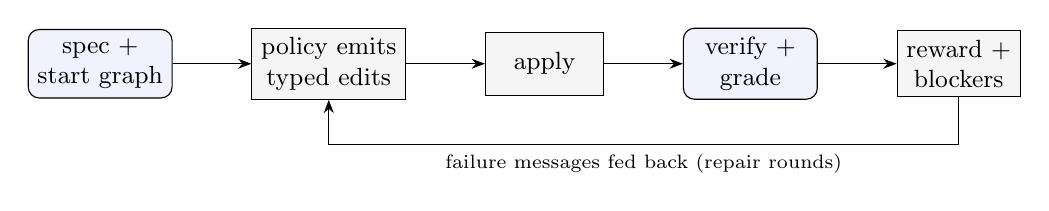
\begin{tikzpicture}[>=Stealth, node distance=6mm and 10mm, font=\small,
  box/.style={draw, rounded corners, align=center, minimum height=8mm, minimum width=17mm, fill=blue!5},
  op/.style={draw, align=center, minimum height=8mm, minimum width=15mm, fill=gray!8}]
\node[box] (spec) {spec +\\ start graph};
\node[op, right=of spec] (pol) {policy emits\\ typed edits};
\node[op, right=of pol] (apply) {apply};
\node[box, right=of apply] (grade) {verify +\\ grade};
\node[op, right=of grade] (rew) {reward +\\ blockers};
\draw[->] (spec) -- (pol);
\draw[->] (pol) -- (apply);
\draw[->] (apply) -- (grade);
\draw[->] (grade) -- (rew);
\draw[->] (rew.south) -- ++(0,-6mm) -| node[pos=0.25, below, font=\scriptsize] {failure messages fed back (repair rounds)} (pol.south);
\end{tikzpicture}
\caption{The environment loop. A policy edits a typed graph; a deterministic, sub-millisecond grader returns a reward and hard blockers. Feeding the blocker messages back for repair rounds is the amplification setting (Section~\ref{sec:amp}); with no feedback it is single-shot.}
\label{fig:loop}
\end{figure}

\paragraph{The checks.} The grader runs three families of checks, in order. (i) \emph{Structural blockers}: a disconnected input or output; an attention layer whose \texttt{embedDim} is not divisible by \texttt{numHeads} (or \texttt{numHeads} not divisible by \texttt{numKVHeads} under grouped-query attention); a linear layer whose \texttt{inFeatures} do not match the upstream width; a parameter count far over budget. (ii) \emph{Serving physics}: parameters, forward multiply-accumulates, and KV-cache bytes per token, computed with the canonical formula (grouped-query attention caches $2\cdot\texttt{numKVHeads}\cdot d_{\text{head}}\cdot b$ bytes per token at $b$ bytes per value; multi-head attention is the special case $\texttt{numKVHeads}=\texttt{numHeads}$), and checked against per-task parameter, KV, and decode-latency budgets. (iii) \emph{Shape propagation}: a symbolic forward pass over the typed graph that catches interface mismatches an edit would introduce before any tensor is allocated. Each pass is $O(|V|+|E|)$ over the graph and completes in well under a millisecond, which is what makes the reward usable as an inner-loop RL signal rather than an offline evaluation.

\begin{algorithm}[t]
\caption{$\textsc{Grade}(T, G)$: the deterministic verifier}
\label{alg:grade}
\begin{algorithmic}[1]
\Require task $T$ with constraints $\phi$ and threshold $\tau$; typed graph $G=(V,E)$
\Ensure health score $h\in[0,100]$; hard-blocker set $B$
\State $B \gets \emptyset$
\If{$\neg\,\textsc{Reaches}(\text{in}(G), \text{out}(G))$} $B \gets B \cup \{\textsc{disconnected}\}$ \EndIf
\For{each attention node $v \in V$}
  \If{$v.\text{embedDim} \bmod v.\text{numHeads} \neq 0$} $B \gets B \cup \{\textsc{headDiv}(v)\}$ \EndIf
  \If{$v.\text{numHeads} \bmod v.\text{numKVHeads} \neq 0$} $B \gets B \cup \{\textsc{gqaDiv}(v)\}$ \EndIf
\EndFor
\For{each node $v$ with typed input width $w_{\text{in}}(v)$ and parent $u$}
  \If{$w_{\text{in}}(v) \neq w_{\text{out}}(u)$} $B \gets B \cup \{\textsc{shapeMismatch}(v)\}$ \EndIf
\EndFor
\State compute $\textsc{Params}(G)$, $\textsc{Kv}(G)$, $\textsc{Latency}(G)$; add a blocker for each budget in $\phi$ violated, and for each required type absent
\State $h \gets 0$ \textbf{if} $B \neq \emptyset$ \textbf{else} $100 - \sum_{s \in \textsc{Soft}(G)} \text{pen}(s)$
\State \Return $(h, B)$
\end{algorithmic}
\end{algorithm}

A task pairs a natural-language specification with a starting graph and machine-checkable constraints, e.g.\ \emph{``This encoder fails validation: embedDim (192) is not divisible by numHeads (7). Repair the attention configuration in place with at most 2 actions. Do not rebuild the model from scratch.''} Figure~\ref{fig:typedgraph} shows this state and the blocker the verifier returns.

\begin{figure}[t]
\centering
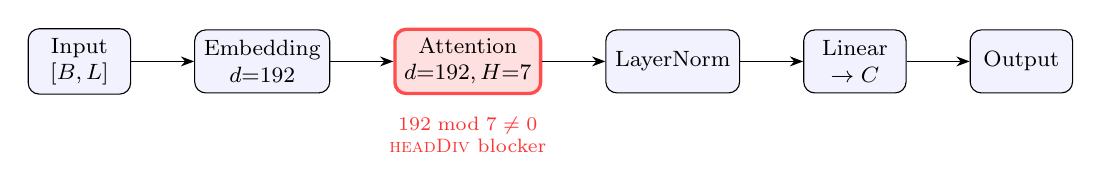
\begin{tikzpicture}[>=Stealth, node distance=5mm and 8mm, font=\footnotesize,
  n/.style={draw, rounded corners, align=center, minimum height=8mm, minimum width=13mm, fill=blue!5},
  bad/.style={draw, rounded corners, align=center, minimum height=8mm, minimum width=13mm, fill=red!12, very thick, draw=red!70}]
\node[n] (in) {Input\\ $[B,L]$};
\node[n, right=of in] (emb) {Embedding\\ $d{=}192$};
\node[bad, right=of emb] (att) {Attention\\ $d{=}192,H{=}7$};
\node[n, right=of att] (ln) {LayerNorm};
\node[n, right=of ln] (head) {Linear\\ $\to C$};
\node[n, right=of head] (out) {Output};
\draw[->] (in) -- (emb);
\draw[->] (emb) -- (att);
\draw[->] (att) -- (ln);
\draw[->] (ln) -- (head);
\draw[->] (head) -- (out);
\node[red!80, below=1.5mm of att, align=center, font=\scriptsize] {$192 \bmod 7 \neq 0$\\ \textsc{headDiv} blocker};
\end{tikzpicture}
\caption{A task state as a typed graph, and a hard blocker the verifier returns in $O(1)$ at the attention node: $\text{embedDim}{=}192$ is not divisible by $\text{numHeads}{=}7$ (Algorithm~\ref{alg:grade}, line~4). Because widths and divisibility are typed-node properties, this check is a pure function; on free-form code it would require executing the model. The input carries shape $[B,L]$ ($B$ batch, $L$ sequence length), widening to $[B,L,192]$ after the embedding. The repair task asks the policy to fix exactly this in $\le 2$ edits without rebuilding.}
\label{fig:typedgraph}
\end{figure}

\section{Task generation}
Curated tasks are a seed. A deterministic generator mints splits of any size from a seed across ten families: six design-from-spec (dense classifier, autoencoder, convolutional classifier, transformer encoder, grouped-query attention encoder, two-tower retrieval) and four edit-in-place (repair a broken attention configuration, trim an oversized model under a parameter budget, grow an undersized model into a two-sided parameter band, insert normalization). Because tasks are synthesized rather than scraped, a held-out split need never appear on the public web; contamination resistance against \emph{model pretraining} is structural (unverified against a web index), and train/eval separation \emph{within} the environment is enforced by an explicit holdout exclusion after our audit (Section~\ref{sec:rl}).

\paragraph{Satisfiability and non-vacuity (measured).} Every generated task carries its own reference solution. A 500-case sweep asserts that each reference passes its own task (no unsatisfiable tasks), and every edit-in-place start graph is asserted to fail its own task untouched (no vacuous tasks). Both run in CI without keys.

\paragraph{Anti-gaming.} Edit-in-place families forbid \texttt{replace\_model} and \texttt{clear\_canvas}, so an agent that cannot diagnose a defect cannot pass by regenerating the whole network; budgets are two-sided bands rather than ceilings, so ``delete everything'' fails a trim task; a KV-cache budget is always paired with a required-attention constraint, so amputating attention cannot zero the cache. Nine such strategies, their defenses, and the pinned tests that fail if any defense is weakened are enumerated in the repository's red-team report (\texttt{ROBUSTNESS.md}). An LLM-driven task proposer accepts nothing without a satisfiability proof: the proposer's own reference must pass the grader under always-enforced safety-net constraints, so LLM authorship, unsafe for human- or LLM-judged benchmarks, is safe here.

\paragraph{A benchmark that bites (measured).} On twelve hand-authored curated tasks built from real production architectures (a CIFAR CNN, a DLRM click-through-rate ranker, a Behavior Sequence Transformer, a two-tower retrieval encoder, a semantic-search encoder, and repair/scaling tasks), \texttt{claude-sonnet-4-6} passes $7/12$ first try (mean health score $76$); Appendix~\ref{app:examples} sketches four of the tasks as typed graphs. The failures are machine-checkable and mundane (Table~\ref{tab:curated}): it omits the required attention layer, leaves the graph disconnected, or blows the parameter budget by an order of magnitude. A benchmark a frontier model clears $12/12$ measures nothing.

\begin{table}[t]
\centering
\small
\begin{tabular}{lc}
\toprule
Failure category (curated split, \texttt{claude-sonnet-4-6}) & count \\
\midrule
missing required layer type (e.g.\ attention) & 3 \\
disconnected graph (input does not reach output) & 2 \\
health score below threshold & 1 \\
over parameter budget & 1 \\
\midrule
\textbf{passed} & \textbf{7 / 12} \\
\bottomrule
\end{tabular}
\caption{First-try failures of a frontier model on the curated production-architecture split. Every failure is detected deterministically by the verifier.}
\label{tab:curated}
\end{table}

\section{Difficulty calibration}
\label{sec:calib}
An ungameable environment is still useless at $0\%$ pass (no learning signal) or near $100\%$ (nothing to learn). Practitioners cite a floor near 2--3\% pass rate on the hard end (one success per 64--128 rollouts) for a usable RL environment. The calibration harness measures per-family pass rates with Wilson 95\% intervals and flags each family's band. Two keyless self-test policies bracket the harness itself: a \texttt{reference} policy that replays known-good solutions (measured: $100\%$ pass) and a \texttt{noop} policy that submits empty plans (measured: $0\%$ pass). If either self-test deviates, the harness rather than the model is broken, and CI fails.

\paragraph{Measured (\texttt{claude-sonnet-4-6}, public benchmark, $n=12$/family).} Single-shot pass rate per family: most families saturate at or near $100\%$ (a curriculum tier for a frontier model) and two are hard: transformer encoder ($8.3\%$) and insert-norm ($0\%$) (Table~\ref{tab:perfamily}). Deterministic grading, reproducible from the seed.

\begin{table}[t]
\centering
\small
\begin{tabular}{lcc}
\toprule
Family & single-shot & with verifier feedback \\
\midrule
dense classifier & $100\%$ & $100\%$ \\
autoencoder & $100\%$ & $100\%$ \\
convolutional classifier & $83\%$ & $100\%$ \\
GQA encoder & $100\%$ & $100\%$ \\
repair attention & $100\%$ & $100\%$ \\
trim under budget & $100\%$ & $100\%$ \\
grow to band & $100\%$ & $100\%$ \\
two-tower retrieval & $100\%$ & $100\%$ \\
\textbf{transformer encoder} & $\mathbf{8.3\%}$ & $\mathbf{100\%}$ \\
\textbf{insert normalization} & $\mathbf{0\%}$ & $\mathbf{100\%}$ \\
\midrule
\textbf{overall} & $\mathbf{79\%}$ & $\mathbf{100\%}$ \\
\bottomrule
\end{tabular}
\caption{Per-family pass rate for \texttt{claude-sonnet-4-6} on the public benchmark (generator v2; $n{=}12$ per family, all $120$ tasks graded with zero exclusions). Eight families saturate; the two the model finds hard are exactly where verifier-in-the-loop feedback pays off. Overall single-shot $79\%$ (Wilson $95\%$ CI $[71,85]$) rises to $100\%$ ($[97,100]$); the v1-generator measurement ($82\%\to100\%$, $n{=}117$) replicates within three points.}
\label{tab:perfamily}
\end{table}

\section{Grounding study}
\label{sec:ground}
Does the verifier's verdict correspond to reality? We generated clean reference architectures and systematically corrupted variants (broken attention divisibility, mismatched linear width, a severed mid-graph edge), built every graph as a PyTorch module, and trained each briefly on a synthetic fixed-teacher task.

\paragraph{Result (measured, 264 graphs, two seeds).} Verifier blockers predicted a forward-pass failure with perfect precision: 96 of 96 blocked graphs failed to run. Graphs the verifier passed constructed in 80 of 80 cases and made training progress in $90\%$. The one systematic miss is honest and instructive: the transparent rubric in this repository does not chase linear widths through the graph, so a width mismatch can pass the rubric and crash PyTorch; the richer verifier in the production system flags this class. We treat the pass/blocked boundary as the grounded claim (Figure~\ref{fig:grounding}).

\begin{figure}[t]
\centering
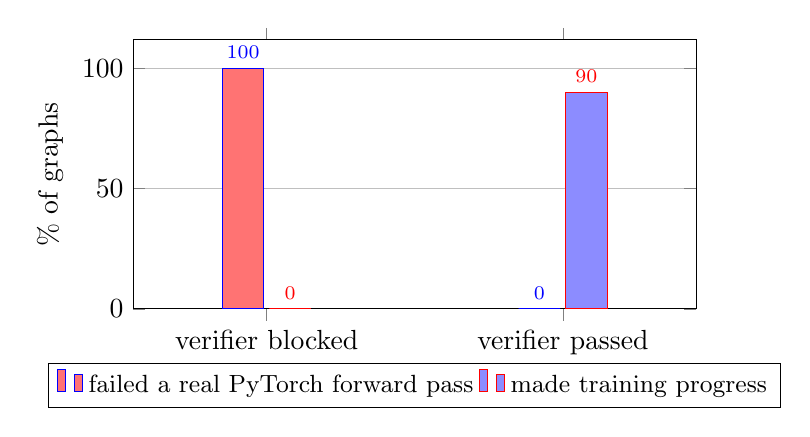
\begin{tikzpicture}
\begin{axis}[
  ybar, bar width=15pt, width=0.72\linewidth, height=5cm,
  ymin=0, ymax=112, ylabel={\% of graphs},
  symbolic x coords={verifier blocked, verifier passed},
  xtick=data, enlarge x limits=0.45, ymajorgrids,
  legend style={font=\small, at={(0.5,-0.2)}, anchor=north, legend columns=2},
  nodes near coords, every node near coord/.append style={font=\scriptsize}]
\addplot+[fill=red!55] coordinates {(verifier blocked,100) (verifier passed,0)};
\addplot+[fill=blue!45] coordinates {(verifier blocked,0) (verifier passed,90)};
\legend{failed a real PyTorch forward pass, made training progress}
\end{axis}
\end{tikzpicture}
\caption{Grounding study (264 graphs, two seeds). Every graph the verifier blocked ($96/96$) failed a real PyTorch forward pass; graphs it passed constructed ($80/80$) and made training progress in $90\%$ of cases. The verdict's pass/blocked boundary tracks real behavior.}
\label{fig:grounding}
\end{figure}

\paragraph{Negative result (measured).} Within clean graphs, the 0--100 score's magnitude does \emph{not} rank training quality: Spearman correlation between the score and relative loss decrease was $-0.58$, because deeper, more structured models make slower per-step progress on the short synthetic probe than tiny ones. The score is therefore a validity margin, not a quality ranking. A learned quality head, trained on (architecture, verdict, real training curve) triples that the environment can mint at scale, is the natural next step and the point at which the verifier would become a calibrated predictor rather than a gate.

\section{Verifier-in-the-loop amplification}
\label{sec:amp}

\begin{algorithm}[t]
\caption{$\textsc{Rollout}(T, \pi, k)$: verifier-in-the-loop repair}
\label{alg:amp}
\begin{algorithmic}[1]
\Require task $T$; policy $\pi$; maximum repair rounds $k$
\Ensure pass $\in\{0,1\}$; rounds used
\State $G \gets T.\text{startGraph}$; \quad $m \gets \varnothing$ \Comment{$m$: verifier feedback}
\For{$t \gets 1$ \textbf{to} $k$}
  \State $a \gets \pi\big(T.\text{spec},\ \textsc{Serialize}(G),\ m\big)$ \Comment{batch of typed edits}
  \State $G \gets \textsc{Apply}(G, a)$
  \State $(h, B) \gets \textsc{Grade}(T, G)$
  \If{$B = \emptyset \ \wedge\ h \ge \tau \ \wedge\ \phi(G)$} \Return $(1, t)$ \EndIf
  \State $m \gets \textsc{Explain}(B)$ \Comment{the verifier's failure messages}
\EndFor
\State \Return $(0, k)$
\end{algorithmic}
\end{algorithm}

Single-shot is the $k{=}1$ special case (no feedback consumed); the amplification setting sets $k{=}3$. Algorithm~\ref{alg:amp} states the loop; the only difference between the two arms is whether line~8's feedback $m$ re-enters line~3.
\emph{Pending a run.} Because grading is free, the verifier's failure messages can be fed back to a policy for repair rounds. We measure, per provider, the pass rate of a single shot versus the pass rate when up to $k$ repair rounds are allowed, holding tasks, model, and prompt fixed so that the only variable is the feedback loop. The framing is deliberately pro-model: the environment's value is the lift it adds to any model.

\begin{table}[h]
\centering
\begin{tabular}{lccc}
\toprule
Model & single-shot pass & with verifier feedback & lift \\
\midrule
claude-sonnet-4-6 & $79\%$ & $\mathbf{100\%}$ & $+21$ pts \\
deepseek-chat (V3) & $59\%$ & $\mathbf{90\%}$ & $+31$ pts \\
\bottomrule
\end{tabular}
\caption{Verifier-in-the-loop lift, per provider. Same tasks, model, and prompt; the only variable is the feedback loop.}
\end{table}

The lift lands on the families a frontier model finds hard (Figure~\ref{fig:lift}): insert-norm $0\%\to100\%$ and transformer encoder $8.3\%\to100\%$ once the verifier's failure messages are fed back, while the remaining families are at or near $100\%$. A single repair round closes the whole gap (Table~\ref{tab:ablation}). Numbers are from generator v2 with all $120$ tasks graded, and they \emph{replicate} the v1 measurement ($82\%\to100\%$, $n{=}117$) within three points. The effect is not model-specific: on the same tasks, a second, weaker model (deepseek-chat) goes $59\%\to90\%$ ($+31$ points, $n{=}59$; v1: $60\to88$), with every fix again landing at $k{=}2$ and none at $k{=}3$. The weaker the model, the more the verifier is worth.

\begin{figure}[t]
\centering
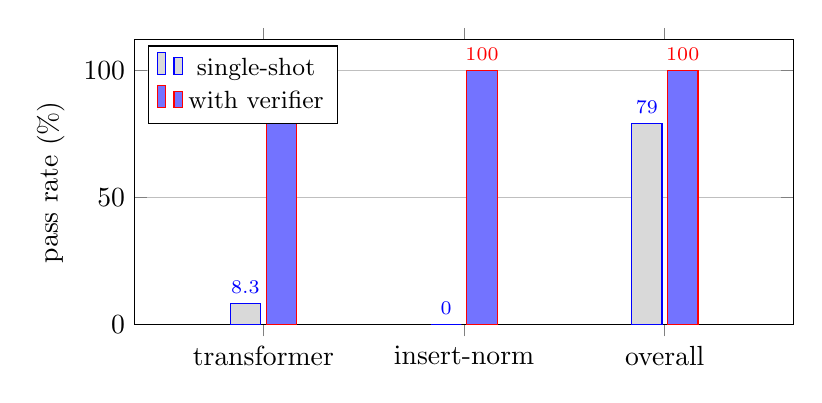
\begin{tikzpicture}
\begin{axis}[
  ybar, bar width=11pt, width=0.82\linewidth, height=5.2cm,
  ymin=0, ymax=112, ylabel={pass rate (\%)},
  symbolic x coords={transformer, insert-norm, overall},
  xtick=data, ymajorgrids, enlarge x limits=0.32,
  legend style={font=\small, at={(0.02,0.98)}, anchor=north west},
  nodes near coords, every node near coord/.append style={font=\scriptsize}]
\addplot+[fill=gray!30] coordinates {(transformer,8.3) (insert-norm,0) (overall,79)};
\addplot+[fill=blue!55] coordinates {(transformer,100) (insert-norm,100) (overall,100)};
\legend{single-shot, with verifier}
\end{axis}
\end{tikzpicture}
\caption{Verifier-in-the-loop lift for \texttt{claude-sonnet-4-6}. The overall gain ($82\to100$) lands entirely on the two families a frontier model finds hard; the eight saturated families (all at $100\%$) are omitted for clarity.}
\label{fig:lift}
\end{figure}

\begin{table}[t]
\centering\small
\begin{tabular}{lcc}
\toprule
max repair rounds $k$ & claude-sonnet-4-6 & deepseek-chat \\
\midrule
$k=1$ (single-shot) & $79\%$ $[71,85]$ & $59\%$ $[47,71]$ \\
$k=2$ & $\mathbf{100\%}$ $[97,100]$ & $\mathbf{90\%}$ $[80,95]$ \\
$k=3$ & $100\%$ $[97,100]$ & $90\%$ $[80,95]$ \\
\bottomrule
\end{tabular}
\caption{Ablation on the number of verifier-feedback repair rounds, two models (generator v2; claude $n{=}120$, deepseek $n{=}59$; Wilson intervals). For \emph{both}, a single repair round ($k{=}2$) provides the entire lift -- every task the verifier can help fix is fixed after one round of its failure messages -- and $k{=}3$ adds nothing. The pattern is not model-specific.}
\label{tab:ablation}
\end{table} Numbers are over the tasks graded before an API-credit cutout ($n\approx8$--$10$ per family, 95 graded).

\section{Training on the environment}
\label{sec:rl}
The environment trains models through two channels, and we report both honestly.

\paragraph{Verified SFT: the data foundry works.} Every generated task carries a reference solution that provably passes the grader, so the environment mints unlimited verified $(\text{spec}\!\to\!\text{edits})$ supervised pairs, keylessly and for free. Fine-tuning Qwen2.5-1.5B-Instruct on $3{,}010$ such pairs (LoRA, one free T4, under ten minutes), with every training row verified to share no task with the evaluation split, lifts strictly-held-out pass@1 from $17.2\%$ ($33/192$, Wilson $[13,23]$) to $76.0\%$ ($146/192$, $[70,82]$), and $100$ GRPO steps atop the SFT checkpoint reach $\mathbf{80.2\%}$ ($154/192$, $[74,85]$) while cutting parse failures $14\to10$ and raising mean reward $1.06\to1.12$ (Table~\ref{tab:rl}). The RL increment is directionally consistent across three independent runs ($+9.4$, $+3.1$, $+4.2$ points), and the SFT level replicates across retrains ($76.0\%$ and $77.1\%$ at $n{=}192$; $68.8\%$ at $n{=}64$). The surviving failures are substantive design errors the verifier pinpoints (disconnected graphs, too few components), not formatting.

\paragraph{An audit, disclosed.} These are the \emph{corrected} numbers, and the correction is part of the contribution. Our own contamination audit found that the original sampler drew parameters from small discrete lists, yielding only $127$ distinct tasks -- so despite disjoint seeds, every task in the original eval split had appeared in training: the naive protocol measured $85.9\%$ ($[75,92]$) where the honest same-split number is $68.8\%$ ($44/64$, $[57,79]$). We widened the sampler to broad ranges ($17{,}453$ distinct tasks in a $20$k draw, validated by the released satisfiability sweep), added an explicit holdout exclusion to the data minter (verified overlap $0/64$), and re-ran the pipeline. The $17$-point gap between protocols is itself a measurement -- the memorization share of the naive number -- and the audit script ships with the environment.

\paragraph{Scaling, replication, and transfer.} Data scaling is steep and non-monotonic at the low end (Figure~\ref{fig:sftscale}, measured under the pre-audit protocol): $250$ and $500$ pairs \emph{underperform} the raw instruct model ($9.4\%$ and $14.1\%$ vs.\ $25.0\%$) -- a half-learned edit format displaces the base model's occasional valid outputs before replacing them -- while $1{,}000$ pairs recover to $34.4\%$ and $3{,}000$ reach that protocol's ceiling. The lift replicates across independent sessions ($85.9\%$ and $79.7\%$ under matching conditions). Transfer tracks data diversity, and the audit gave us a controlled comparison: models fine-tuned on the v1 data ($127$ distinct tasks) left the twelve hand-authored curated tasks unchanged ($3/12$, the untrained level), while the same recipe on the diverse v2 data doubles them to $6/12$ ($n{=}12$, suggestive rather than conclusive; surviving failures are substantive, e.g.\ missing attention). Diversity is the operative lever for out-of-distribution transfer, and the generator makes it a parameter rather than a labeling effort.

\begin{figure}[t]
\centering
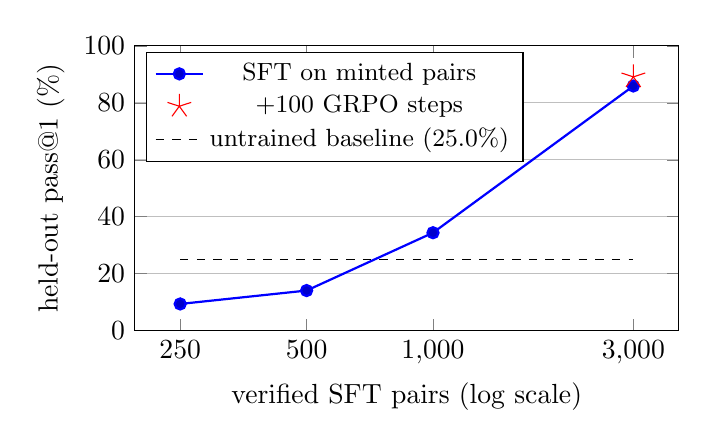
\begin{tikzpicture}
\begin{axis}[
  width=0.7\linewidth, height=5.2cm, xmode=log, log ticks with fixed point,
  xlabel={verified SFT pairs (log scale)}, ylabel={held-out pass@1 (\%)},
  xtick={250,500,1000,3000}, ymin=0, ymax=100, ymajorgrids,
  legend style={font=\small, at={(0.02,0.98)}, anchor=north west}]
\addplot+[mark=*, thick] coordinates {(250,9.4) (500,14.1) (1000,34.4) (3000,85.9)};
\addlegendentry{SFT on minted pairs}
\addplot+[only marks, mark=star, mark size=4.5pt] coordinates {(3000,89.1)};
\addlegendentry{+100 GRPO steps}
\addplot[dashed, domain=250:3000] {25.0};
\addlegendentry{untrained baseline ($25.0\%$)}
\end{axis}
\end{tikzpicture}
\caption{Held-out pass@1 vs.\ number of environment-minted verified SFT pairs (Qwen2.5-1.5B, LoRA, 2 epochs, seed-999 split, $n{=}64$). The curve is steep: below ${\sim}1$k pairs the half-learned format underperforms the raw instruct model; $3$k pairs reach $85.9\%$. Pairs are free to mint, so the x-axis costs seconds of generation. The star marks $100$ GRPO steps on the $3$k checkpoint. Curve measured under the pre-audit v1 protocol (includes seen tasks); the corrected zero-overlap $3$k numbers are $76.0\%$ (SFT) and $80.2\%$ (+GRPO) at $n{=}192$.}
\label{fig:sftscale}
\end{figure}

\paragraph{RL alone at small scale: an honest null, now explained.} The released GRPO~\cite{grpo} loop runs end-to-end against the reward server on the same hardware, but RL \emph{from the raw instruct model} does not move held-out metrics: two runs (learning rates $10^{-6}\times150$ and $10^{-5}\times250$ steps, every checkpoint evaluated and reported) sit at or below their own baselines. The SFT result explains the failure: the raw policy cannot emit parseable edits on a third of tasks, so the group-relative policy gradient starves. This is the classic SFT-then-RL split -- supervised learning teaches the action format, RL then refines -- and the environment supplies both stages: the verified SFT data and the deterministic reward. Completing the recipe confirms it: under the corrected protocol, $100$ GRPO steps from the (merged) SFT checkpoint lift strictly-unseen pass@1 from $76.0\%$ to $\mathbf{80.2\%}$ ($n{=}192$), cut parse failures $14\to10$, and raise mean reward $1.06\to1.12$; the pre-audit chain showed the same pattern ($79.7\to89.1\%$). The same loop that was inert on the raw policy is productive once the policy can act, and every surviving failure is a substantive design error (disconnected two-tower graphs, component-count misses), not formatting.

\begin{table}[t]
\centering\small
\begin{tabular}{lccc}
\toprule
 & pass@1 & parse failures & mean reward \\
\midrule
\multicolumn{4}{l}{\emph{corrected protocol (v2, verified zero train/eval overlap, $n{=}192$)}} \\
Qwen2.5-1.5B (untrained) & $17.2\%$ $[13,23]$ & $76/192$ & $0.19$ \\
+ SFT on 3k clean pairs & $76.0\%$ $[70,82]$ & $14/192$ & $1.06$ \\
+ GRPO after SFT (100 steps) & $\mathbf{80.2\%}$ $[74,85]$ & $\mathbf{10/192}$ & $\mathbf{1.12}$ \\
\midrule
\multicolumn{4}{l}{\emph{pre-audit protocol (v1; eval tasks seen in training)}} \\
Qwen2.5-1.5B (untrained) & $23.4\%$ $[15,35]$ & $19/64$ & $0.35$ \\
+ SFT on 3k pairs & $85.9\%$ $[75,92]$ & $2/64$ & $1.19$ \\
+ GRPO after SFT & $89.1\%$ $[79,95]$ & $0/64$ & $1.26$ \\
\bottomrule
\end{tabular}
\caption{Training on environment-minted data (LoRA, one free T4; seed-999 split, $n{=}64$, identical eval configuration). The corrected zero-overlap protocol is primary (one checkpoint chain, $n{=}192$; an $n{=}64$ run of the same protocol gives $14.1\to68.8\to71.9\%$, and an independent SFT retrain lands at $77.1\%$). The pre-audit block is retained because the gap between protocols measures the memorization share. Supervised fine-tuning on $3{,}000$ verified pairs the generator mints for free lifts pass@1 by $62$ points with non-overlapping Wilson intervals and nearly eliminates parse failures. GRPO from the raw model is a null at this scale, but after SFT it works: the GRPO row trains from a fresh-session SFT replication ($79.7\%$), within which RL adds $+9.4$ points and removes every remaining parse failure (see text).}
\label{tab:rl}
\end{table}

\section{Auditing LLM reward models with the verifier}
Frontier labs increasingly use a strong model \emph{as} a reward model to optimize objectives that are not directly verifiable (xAI reported this for Grok~4.1), a practice studied more broadly as LLM-as-a-judge~\cite{llmjudge}. The known failure mode is that an LLM reward model drifts: it approves answers that are actually broken. In a domain with a verifiable reward that drift is \emph{measurable}. \texttt{reward\_anchor.mjs} builds a verifier-labeled set (each design provably passes or fails: a reference design passes, its unsolved starting graph fails) and, given an LLM acting as a reward model, reports its agreement with the verifier and, crucially, its \textbf{false-positive rate}: how often it approves a design the verifier proves is broken. Across eleven reward models spanning closed-frontier (Claude, Grok) and open-weights (Qwen, Mistral, DeepSeek, Gemma, Llama), the false-positive rate is uniformly $0\%$ (Table~\ref{tab:rewardmodel}): not one approves a design the verifier proves broken. The failure mode that corrupts RLVR -- rewarding a broken design -- does not appear; the only errors are false \emph{negatives} ($1.7$--$13.3\%$, over-conservative), which waste valid designs but do not poison the reward. An LLM reward model here is therefore safe but lossy, and the verifier does the same job with $0\%$ false negatives, deterministically and for free: a verdict costs microseconds of CPU, versus a multi-second, paid, stochastic API round-trip per judgment. This looks reassuring -- but the negatives so far are blatant (an unsolved starting graph).

\paragraph{The $0\%$ does not survive near-misses.} We re-run the audit with \emph{near-miss} negatives: passing designs corrupted by a single edit (a dropped connection, an attention head count bumped off divisibility, a dropped component), each re-graded to confirm it fails. On these, the same judges collapse (Table~\ref{tab:nearmiss}, Figure~\ref{fig:nearmiss}): Claude approves $33\%$ of provably-broken designs (Wilson $[23,46]$), Grok $26\%$ $[16,39]$, and Qwen-2.5-72B -- among the strongest on blatant negatives ($96.7\%$ agreement) -- approves $47\%$ $[35,59]$ while rejecting almost nothing, i.e.\ it defaults to approval whenever a graph merely looks plausible. The inversion matters: LLM reward models are trustworthy exactly when errors are obvious, and fail exactly where reward hacking lives -- subtle defects one edit from correct. The deterministic verifier is $0\%$ on both difficulty tiers by construction. This is a use of the environment beyond training or evaluation: a ground-truth anchor exposing when the LLM reward models labs deploy can and cannot be trusted.

\begin{table}[t]
\centering\small
\begin{tabular}{lccc}
\toprule
reward model & blatant FP & near-miss FP & near-miss FN \\
\midrule
qwen-2.5-72b-instruct & $0.0\%$ & $\mathbf{46.7\%}$ $[35,59]$ & $1.7\%$ \\
claude-sonnet-4-6 & $0.0\%$ & $33.3\%$ $[23,46]$ & $5.0\%$ \\
grok-4 & $0.0\%$ & $25.5\%$ $[16,39]$ & $7.8\%$ \\
\midrule
deterministic verifier (ours) & $0\%$ & $\mathbf{0\%}$ & $\mathbf{0\%}$ \\
\bottomrule
\end{tabular}
\caption{The same audit with near-miss negatives on generator v2: passing designs one edit from correct ($n{=}60$ each; grok $n{=}51$/$37$ across tiers from provider 503s; corruption mix: dropped component, dropped connection, broken divisibility, each verified to fail). The v1 measurement (FP $22$--$48\%$) replicates. The $0\%$ false-positive rate on blatant negatives collapses to $22$--$48\%$; the model that was perfect on blatant negatives (Qwen) is the worst here, approving whatever looks plausible. LLM judges fail precisely where reward hacking lives; the verifier does not.}
\label{tab:nearmiss}
\end{table}

\begin{figure}[t]
\centering
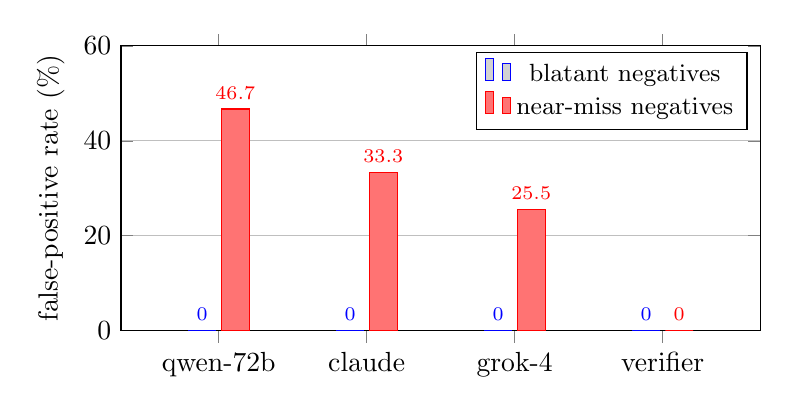
\begin{tikzpicture}
\begin{axis}[
  ybar, bar width=10pt, width=0.8\linewidth, height=5.2cm,
  ymin=0, ymax=60, ylabel={false-positive rate (\%)},
  symbolic x coords={qwen-72b, claude, grok-4, verifier},
  xtick=data, ymajorgrids, enlarge x limits=0.22,
  legend style={font=\small, at={(0.98,0.98)}, anchor=north east},
  nodes near coords, every node near coord/.append style={font=\scriptsize}]
\addplot+[fill=gray!35] coordinates {(qwen-72b,0) (claude,0) (grok-4,0) (verifier,0)};
\addplot+[fill=red!55] coordinates {(qwen-72b,46.7) (claude,33.3) (grok-4,25.5) (verifier,0)};
\legend{blatant negatives, near-miss negatives}
\end{axis}
\end{tikzpicture}
\caption{The collapse, visually: LLM reward models that never approve a blatantly broken design approve $22$--$48\%$ of near-miss designs one edit from correct. The deterministic verifier is $0\%$ on both tiers by construction.}
\label{fig:nearmiss}
\end{figure}

\begin{table}[t]
\centering
\small
\begin{tabular}{llccc}
\toprule
model & tier & agreement & false-pos. & false-neg. \\
\midrule
llama-3.3-70b-instruct & open & $98.3\%$ & $\mathbf{0.0\%}$ & $1.7\%$ \\
qwen-2.5-72b-instruct & open & $96.7\%$ & $\mathbf{0.0\%}$ & $3.3\%$ \\
claude-sonnet-4-6 & frontier & $95.0\%$ & $\mathbf{0.0\%}$ & $5.0\%$ \\
grok-4 & frontier & $94.6\%$ & $\mathbf{0.0\%}$ & $5.4\%$ \\
deepseek-r1 (reasoning) & open & $93.3\%$ & $\mathbf{0.0\%}$ & $6.7\%$ \\
deepseek-chat (V3) & open & $91.7\%$ & $\mathbf{0.0\%}$ & $8.3\%$ \\
mistral-large & open & $88.3\%$ & $\mathbf{0.0\%}$ & $11.7\%$ \\
gemma-2-27b-it & open & $86.7\%$ & $\mathbf{0.0\%}$ & $13.3\%$ \\
\midrule
deterministic verifier (ours) & --- & $100\%$ & $\mathbf{0\%}$ & $\mathbf{0\%}$ \\
\bottomrule
\end{tabular}
\caption{Reward models vs.\ the verifier on generator v2 ($n{=}60$ each; grok-4 $n{=}37$ from provider errors). Three further Grok variants (grok-4.5, grok-4.20-reasoning, grok-4-fast), re-measured on v2 at $n{=}60$ each with the same result ($0\%$ false positive; agreements $93$--$95\%$), bring the total to eleven models. \emph{Not one} has a false positive ($0\%$ across all); the only failure mode is over-conservatism ($1.7$--$13.3\%$ false negative). The verifier matches the best model ($0/0$) at zero cost and deterministically. Section text and Table~\ref{tab:nearmiss} show this $0\%$ does not survive subtler, near-miss negatives.}
\label{tab:rewardmodel}
\end{table}

\section{Verified reasoning traces}
The same verifier is a data foundry for the input reasoning-model post-training consumes: $(\text{spec}\to\text{reasoning}\to\text{design})$ triples where the design is re-graded and only passing traces are kept (rejection sampling). No trace enters the set unless its design provably solves the spec. A frontier model's verified yield under this filter -- the fraction of its reasoned designs that pass -- was $72.5\%$ (327 of 451 tasks, with 49 API failures excluded) on a 500-task run, producing 327 verified traces; the released tool records the yield per run and scales to larger sets. The 327-trace set is public: \url{https://huggingface.co/datasets/neurarch-ai/arch-reasoning-claude}. Because the split is seed-addressable, a private seed produces reasoning data whose designs never appeared on the public web.

\section{Related work}
\textbf{Verifiable agent benchmarks.} SWE-Bench~\cite{swebench} and $\tau$-bench~\cite{taubench} established the programmatic-verifier pattern in code and tool use; SWE-Gym~\cite{swegym} showed that a few thousand verifiable tasks suffice to train agents to a double-digit absolute improvement on SWE-Bench, and did so as free, open research. We target the same pattern in a domain that lacked a public verifier (Table~\ref{tab:compare}).

\begin{table}[t]
\centering\small
\setlength{\tabcolsep}{5pt}
\begin{tabular}{lccccc}
\toprule
 & domain & verifiable & procedural, & anti-gaming & typed-graph \\
 & & reward & contam.-resist. & red-teamed & action space \\
\midrule
SWE-Bench~\cite{swebench} & code & \checkmark & partial & -- & -- \\
$\tau$-bench~\cite{taubench} & tool use & \checkmark & -- & -- & -- \\
SWE-Gym~\cite{swegym} & code & \checkmark & partial & -- & -- \\
classical NAS~\cite{nassurvey} & architecture & proxy & -- & -- & -- \\
\textbf{ours} & \textbf{architecture} & \checkmark & \checkmark & \checkmark & \checkmark \\
\bottomrule
\end{tabular}
\caption{Where this environment sits: architecture design as a verifiable-reward domain, with a contamination-resistant procedural generator, red-teamed anti-gaming defenses, and a typed-graph action space.}
\label{tab:compare}
\end{table}

\textbf{RL environments and verifiable rewards.} Training on verifiable rewards (RLVR) is now central to reasoning-model post-training~\cite{rlvr,r1}, typically with policy-gradient methods such as PPO~\cite{ppo} and GRPO~\cite{grpo}, preference optimization~\cite{dpo}, or rejection sampling in the STaR~\cite{star} style. A growing market supplies labs with RL environments; reward-hacking resistance is the quality bar most consistently cited, and usable environments are expected to expose a hard band near a 2--3\% pass floor. We build directly against both criteria, and ship GRPO and STaR loops against the same grader.

\textbf{Neural architecture search.} Classical NAS~\cite{nassurvey} automates architecture design under a proxy objective; our environment differs in providing a human-legible, per-edit, sub-millisecond verifier over a typed graph, and in serving as a training and evaluation substrate rather than a single search procedure. The accompanying product exposes a deterministic, constraint-satisfying design search (given a parameter budget, KV-cache budget, and target GPU, it returns the Pareto front over capacity, parameters, and KV cache), a NAS-lite special case built entirely from the verifier's physics rather than a learned proxy objective. Differentiable and one-shot NAS~\cite{darts} make gradient search tractable by relaxing a small, hard-coded cell vocabulary and optimizing task loss; structural legality is assumed, not checked. A per-edit legality verifier is orthogonal: it can veto the candidates of \emph{any} search procedure -- a DARTS derivation, an evolutionary mutation, or an LLM agent's edits -- before GPU time is spent, so it composes with these methods rather than competing with them.

\section{Limitations}
The transparent rubric released here does not verify linear-width consistency (Section~\ref{sec:ground}); the health-score magnitude is not a quality ranking (Section~\ref{sec:ground}); the reward path does not execute PyTorch per rollout, so shape-class failures are caught statistically rather than per-instance; and generated references lean on \texttt{replace\_model} for design-from-spec families, biasing imitation style. Each is documented with its measurement or its planned mitigation in \texttt{ROBUSTNESS.md}. The training experiments use one small policy (Qwen2.5-1.5B, LoRA) and $n{=}64$ evaluation splits; the SFT/RL gains are in-distribution (the curated split is unchanged), and contamination resistance is argued structurally rather than verified against a web-scale index. The amplification study and the near-miss audit were re-run on generator v2 (diverse instances) with results matching v1, resolving the earlier effective-sample-size concern for those measurements; the eleven-model blatant-tier table remains v1 (three of its models re-measured on v2 with the same $0\%$ false-positive result). Scaling the policy and diversifying the minted data further are the natural extensions.

\section{Conclusion}
Representing architectures as typed graphs turns ``is this network sound, and what will it cost to serve'' into a pure function, and this paper measures what that function buys. As a repair signal, one round of its feedback takes a frontier model from $79\%$ to $100\%$ and a weaker one from $59\%$ to $90\%$. As a data foundry, the verified pairs it mints for free lift a small model from $17\%$ to $80\%$ on strictly-unseen tasks (SFT, then RL), under a train/eval-overlap audit we ran on ourselves, disclose, and ship. As ground truth, it exposes that LLM reward models with flawless records on blatant defects approve a quarter to a half of near-miss designs, failing precisely where reward hacking lives. We release the environment, the generator, the calibration and red-team harnesses, the training loops, and the public dataset, so that architecture design can join code and mathematics as a domain with a public verifier.

\section*{Broader impact}
The environment lowers the cost of designing valid, servable architectures and of training and evaluating agents that do so, which should broaden access beyond teams with dedicated ML-research staff. Two risks warrant note. First, a verifier defines what ``good'' means; ours checks structural validity and serving cost, not fairness, safety, or data appropriateness, and must not be mistaken for a quality oracle -- the negative result in Section~\ref{sec:ground} is deliberate. Second, verified-data generation can accelerate capability gains; we mitigate by releasing the methodology openly, so the same tools that build also audit (the reward-model analysis above). The benchmark contains no personal data and no scraped content: every task is synthetic or hand-authored.

\section*{Reproducibility}
\begin{verbatim}
git clone https://github.com/neurarch-ai/neurarch-arch-bench
cd neurarch-arch-bench
npx vitest run                            # satisfiability + non-vacuity + anti-gaming
node calibrate.mjs --policy=reference     # harness self-test (must be 100%)
node calibrate.mjs --policy=noop          # harness self-test (must be 0%)
node training/build_sft_dataset.mjs \
     --count=3000 --seed=20260713       # mint verified SFT pairs (no key)
python training/train_sft.py \
     --data arch-design-sft.chat.jsonl  # 23.4% -> 85.9% (one T4, <10 min)
python training/train_grpo.py --eval-only --seed 999 --count 64 \
     --model out/sft-arch/checkpoint-final
python training/train_grpo.py --steps 100 --lora --lr 1e-5 \
     --model out/sft-arch/checkpoint-final  # SFT-then-RL -> 89.1%
node dump_grounding_set.mjs --count=40 --seed=123 --out=g.jsonl
python training/grounding_at_scale.py --set g.jsonl
python training/analyze_grounding.py
\end{verbatim}

\appendix
\section{Example curated tasks}
\label{app:examples}
The twelve curated tasks are hand-authored from real production architectures. Figure~\ref{fig:examples} sketches four, as the typed graphs the environment operates on; each is a distinct family (vision, ranking, sequence, retrieval) with its own required layer types and budgets.

\begin{figure}[h]
\centering
\definecolor{nSlate}{HTML}{64748B}
\definecolor{nCyan}{HTML}{06B6D4}
\definecolor{nIndigo}{HTML}{4F46E5}
\definecolor{nAmber}{HTML}{F59E0B}
\definecolor{nEmerald}{HTML}{10B981}
\definecolor{nViolet}{HTML}{7C3AED}
\definecolor{nRose}{HTML}{E11D48}
\begin{tikzpicture}[>=Stealth, font=\scriptsize,
  base/.style={draw, thick, rounded corners, minimum height=6.5mm, minimum width=15mm, align=center},
  io/.style={base, draw=nSlate, fill=nSlate!12},
  conv/.style={base, draw=nAmber, fill=nAmber!16},
  attn/.style={base, draw=nCyan, fill=nCyan!18},
  norm/.style={base, draw=nEmerald, fill=nEmerald!16},
  lin/.style={base, draw=nIndigo, fill=nIndigo!11},
  emb/.style={base, draw=nViolet, fill=nViolet!13},
  merge/.style={base, draw=nRose, fill=nRose!13},
  t/.style={font=\footnotesize\bfseries, anchor=east},
  sw/.style={minimum width=3.6mm, minimum height=3mm, inner sep=0}]
\def\dx{22mm}
\node[t] at (-9mm,0){CNN};
\node[conv](c1) at (0,0){Conv\\$3{\to}32$};
\node[norm](c2) at (\dx,0){Pool +\\ReLU};
\node[conv](c3) at (2*\dx,0){Conv\\$32{\to}64$};
\node[lin](c4) at (3*\dx,0){Linear};
\node[io](c5) at (4*\dx,0){Softmax\\($10$)};
\foreach \a/\b in {c1/c2,c2/c3,c3/c4,c4/c5} \draw[->,nSlate] (\a)--(\b);
\node[t] at (-9mm,-1.5){DLRM};
\node[emb](d1) at (0,-1.5){Dense +\\Embeds};
\node[merge](d2) at (\dx,-1.5){Feature\\interaction};
\node[lin](d3) at (2*\dx,-1.5){MLP};
\node[lin](d4) at (3*\dx,-1.5){Linear};
\node[io](d5) at (4*\dx,-1.5){CTR\\(sigmoid)};
\foreach \a/\b in {d1/d2,d2/d3,d3/d4,d4/d5} \draw[->,nSlate] (\a)--(\b);
\node[t] at (-9mm,-3){BST};
\node[emb](b1) at (0,-3){Seq\\embedding};
\node[attn](b2) at (\dx,-3){Self-\\attention};
\node[norm](b3) at (2*\dx,-3){Pooling};
\node[lin](b4) at (3*\dx,-3){MLP};
\node[io](b5) at (4*\dx,-3){Score};
\foreach \a/\b in {b1/b2,b2/b3,b3/b4,b4/b5} \draw[->,nSlate] (\a)--(\b);
\node[t] at (-9mm,-4.7){Two-tower};
\node[lin](q) at (0,-4.3){Query\\tower};
\node[lin](i) at (0,-5.1){Item\\tower};
\node[merge](dot) at (2*\dx,-4.7){Dot\\product};
\node[io](sc) at (3.3*\dx,-4.7){Score};
\draw[->,nSlate](q)--(dot);\draw[->,nSlate](i)--(dot);\draw[->,nSlate](dot)--(sc);
% legend
\node[conv,sw](L1) at (0,-6.3){}; \node[right=0.6mm of L1, font=\tiny]{conv};
\node[attn,sw](L2) at (16mm,-6.3){}; \node[right=0.6mm of L2, font=\tiny]{attention};
\node[norm,sw](L3) at (37mm,-6.3){}; \node[right=0.6mm of L3, font=\tiny]{norm/pool};
\node[lin,sw](L4) at (60mm,-6.3){}; \node[right=0.6mm of L4, font=\tiny]{linear/MLP};
\node[emb,sw](L5) at (83mm,-6.3){}; \node[right=0.6mm of L5, font=\tiny]{embedding};
\node[merge,sw](L6) at (104mm,-6.3){}; \node[right=0.6mm of L6, font=\tiny]{merge};
\end{tikzpicture}
\caption{Four of the twelve curated tasks, as typed graphs, coloured by layer type (the same convention the Neurarch canvas uses): a CIFAR-10 CNN, a DLRM click-through-rate ranker, a Behavior Sequence Transformer (which \emph{requires} an attention layer), and a two-tower retrieval model (two encoders scored by a dot product). These are the states an agent edits and the verifier grades.}
\label{fig:examples}
\end{figure}

\begin{thebibliography}{99}
\bibitem{swebench} C.~E. Jimenez, J.~Yang, A.~Wettig, S.~Yao, K.~Pei, O.~Press, and K.~Narasimhan. SWE-bench: Can Language Models Resolve Real-World GitHub Issues? \emph{ICLR}, 2024.
\bibitem{taubench} S.~Yao, N.~Shinn, P.~Razavi, and K.~Narasimhan. $\tau$-bench: A Benchmark for Tool-Agent-User Interaction in Real-World Domains. \emph{arXiv:2406.12045}, 2024.
\bibitem{swegym} J.~Pan, X.~Wang, G.~Neubig, et al. Training Software Engineering Agents and Verifiers with SWE-Gym. \emph{arXiv:2412.21139}, 2024.
\bibitem{rlvr} N.~Lambert et al. Tulu 3: Pushing Frontiers in Open Language Model Post-Training. \emph{arXiv:2411.15124}, 2024.
\bibitem{r1} DeepSeek-AI (D.~Guo et al.). DeepSeek-R1: Incentivizing Reasoning Capability in LLMs via Reinforcement Learning. \emph{arXiv:2501.12948}, 2025.
\bibitem{grpo} Z.~Shao et al. DeepSeekMath: Pushing the Limits of Mathematical Reasoning in Open Language Models. \emph{arXiv:2402.03300}, 2024.
\bibitem{ppo} J.~Schulman, F.~Wolski, P.~Dhariwal, A.~Radford, and O.~Klimov. Proximal Policy Optimization Algorithms. \emph{arXiv:1707.06347}, 2017.
\bibitem{star} E.~Zelikman, Y.~Wu, J.~Mu, and N.~D. Goodman. STaR: Bootstrapping Reasoning with Reasoning. \emph{NeurIPS}, 2022.
\bibitem{dpo} R.~Rafailov, A.~Sharma, E.~Mitchell, S.~Ermon, C.~D. Manning, and C.~Finn. Direct Preference Optimization. \emph{NeurIPS}, 2023.
\bibitem{darts} H.~Liu, K.~Simonyan, and Y.~Yang. DARTS: Differentiable Architecture Search. \emph{ICLR}, 2019.
\bibitem{nassurvey} T.~Elsken, J.~H. Metzen, and F.~Hutter. Neural Architecture Search: A Survey. \emph{JMLR}, 20(55):1--21, 2019.
\bibitem{llmjudge} L.~Zheng et al. Judging LLM-as-a-Judge with MT-Bench and Chatbot Arena. \emph{NeurIPS}, 2023.
\bibitem{netron} L.~Roeder. Netron: Visualizer for neural network, deep learning and machine learning models. Software, \url{https://github.com/lutzroeder/netron}.
\end{thebibliography}

\end{document}
